\chapter{Introduction to Network Theory}\label{Network_Theory}

%Networks are all around us, shaping the very fabric of our world. 
From social interactions and transportation systems to the intricate connections within biological organisms and the internet, networks provide a powerful framework to understand complex systems. Graph theory, the mathematical foundation of network theory, offers the tools needed to analyze these interconnected structures.

In this chapter, we introduce the fundamental concepts of network and graph theory, along with various types of random graphs.
Then, we focus on random walks and diffusion processes on networks, considering both classical and quantum cases, which play a crucial role in modeling real-world phenomena such as information spread, epidemic modeling, and quantum transport.


\section{Introduction to Graph Theory}

%definition of network, adjacency matrix, laplacian matrix, shortest path, ...
The mathematical framework used in Network theory is given by Graph theory. 

A graph is defined by an ordinate couple $(V,E)$ where $V = \{1,2,3, ...,n\}$ is the set of nodes or vertices and $E = \left\{ (i, j): i , j \in V ; i \text{ is linked to } j\right\}$ is the set of links or edges. Usually, a general graph is denoted as $G =(N,M)$ where $N$ and $M$ are the cardinality of $V$ and $E$ respectively.

A graph can be viewed also via a $N\times N$ matrix called Adjacency matrix which is defined as
\begin{equation}
    A_{ij}= \left\{ \begin{aligned}
        +1 &\quad \mathrm{if} \; i \; \mathrm{is ~linked ~to} \; j \\
        0 &\quad \mathrm{otherwise} \\
    \end{aligned} \right.  .
\end{equation}
The degree $d_i$ of a node $i$ is the number of nodes to which it is connected. We can introduce the degree matrix $D$ as $D_{ij} = d_i\delta_{ij}$
It can be computed from the adjacency matrix as
\begin{equation}
    d_i = \sum_j A_{ij}.
\end{equation}

Graphs can be grouped mainly into two type: \textit{undirected} and \textit{directed} graph. In the first one if the node $i$ is linked to $j$ then $j$ is linked to $i$, namely $(i, j) = (i, j)$; its adjacency matrix is symmetric.
In contrast, in the second one, if the node $i$ is linked to $j$ not necessary $j$ is linked to $i$, namely $(i, j) \neq (i, j)$; its adjacency matrix is not symmetric.

An important concept in graph theory is the study of connections between nodes that are not directly linked by an edge. As a matter of fact, two nodes can be connected by passing through multiple other nodes.
A \textit{walk} of length $k$ from node $i$ to node $j$ is a sequence of nodes $(x_0,x_1,...,x_k)$ such that $x_0=i$, $x_k=j$ and $(x_l, x_{l+1}) \in E$ for all $l \in \{0, ..., k-1\}$. A node can be crossed multiple times.  
If a walk visits each node only once, it is called a \textit{path}.
A particularly important concept is the \textit{shortest path} or \textit{geodesic} that is the path that crosses the minimum number of nodes.  
The number of walks $W_{ij}(k)$ of length $k$ from node $i$ to node $j$ can be computed using the adjacency matrix as
\begin{equation}
    W_{ij}(k) = (A^k)_{ij} .
\end{equation}

A graph is said to be \textit{connected} if, for each pair of distinct nodes $i$ and $j$, there exists a walk that connects them. 
We can defined $G' =(V',E')$ a subgraph of $G= (V,E)$ if $V' \subseteq V$ and $E' \subseteq E$.
A \textit{component} of a graph $G= (V,E)$ is a connected subgraph $G' =(V',E')$ meaning that not connected to any external node of the graph, that is $(i,j)\notin E$ for each $i\in V'$ and $j\in V\setminus V'$. 
A important concept is the \textit{giant component}: a connected subgraph that has approximately the same number of nodes of the total graph. 

A directed graph is said \textit{irreducible} if its adjacency matrix is not similar by permutation to a block upper triangular matrix. In other word, that exchanging two or more raws the adjacency matrix such that the it can be written in the form
\begin{equation}
    A = \begin{pmatrix}
        A_{11} & A_{12} & \cdots & A_{1N}\\
        0 & A_{22}& \cdots & A_{2N}\\
        \vdots & \vdots & \ddots & \vdots\\
        0 &0 &\cdot & A_{NN}\\
    \end{pmatrix} .
\end{equation}
If it hold, the graph is said \textit{strongly connected}: there exists a path that connect each the nodes to all the other ones.

Some systems present interactions with different strength between the elements. Thus, the binary representation, the link exist or not, is no more sufficient. To model this kind of system we introduce the \textit{weight graphs} $G(V,E,W)$, where $W$ is the set of real weights attached to the links.   
It can be described with the $N\times N$ weight matrix which entries are the weight $w_{ij}$ of each link. If there is no link between two nodes $w_{ij} = 0$. The weight matrix is not necessary symmetric. 

Figure \ref{fig:weight_graphs} shows three examples for undirected, directed and weight networks.
\begin{figure}[ht!]
    \centering
    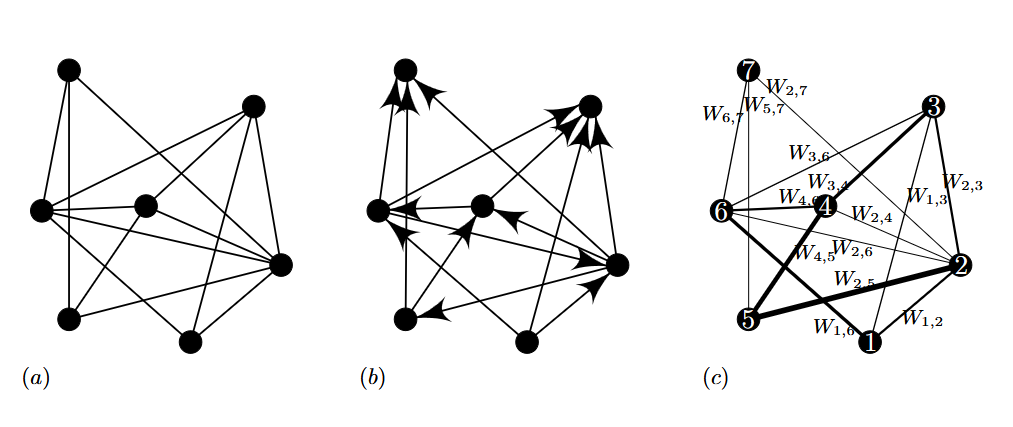
\includegraphics[scale=0.45]{image/weight_graphs.png}
    \caption{Examples of undirected (a), directed (b), weight (c) networks with $N=7$ and $M=13$. The arrows indicates the direction of each link. In the weight graph the thickness of the links represents its weight.}
    \label{fig:weight_graphs}
\end{figure}

\section{Random Networks}
In network theory, random networks play a crucial role in understanding the structure and behavior of complex systems. These networks are often used to model real-world networks, such as the Internet and social networks. There are several methods to generate random networks, each with its own specific focus, such as the degree distribution, the average path length, or the presence of particular structural properties. In this section, we will explore some of the most important models used to generate random networks, highlighting their characteristics and differences.

\subsection{Erd\H{o}s-Rényi Random Graph}

The Erd\H{o}s-Rényi (E-R) random graph $G(N,M)$, where $N$ and $M$ are the number of nodes and links respectively, is one of the first attempts to generate a random network \cite{erdos-renyi1960}. The network is built by randomly choosing $M$ links from all the possible ones. Usually, is used the variation proposed by Gilbert $G(N,p)$ \cite{gilbert} , where $p$ is the probability that two distinct node are connected. The two formulations converge in the thermodynamic limit $N \rightarrow \infty$ and they are interchangeable.
This type of random graph has peculiar properties, such as the degree distribution of the nodes $P(k)$ is binomial
\begin{equation}
    P(k) = \binom{n-1}{k}p^k(1-p)^{n-1-k}
\end{equation} 
Additionally, if $p > \frac{1}{N}$ then is almost sure that the network presents a giant component.
In this work we use the second approach. Figure \ref{E-R_example} shows two examples of E-R random graph, one below and one above the giant component threshold.

\begin{figure}[ht!]
    \centering
    \begin{subfigure}[t]{0.49\textwidth}
        \centering
        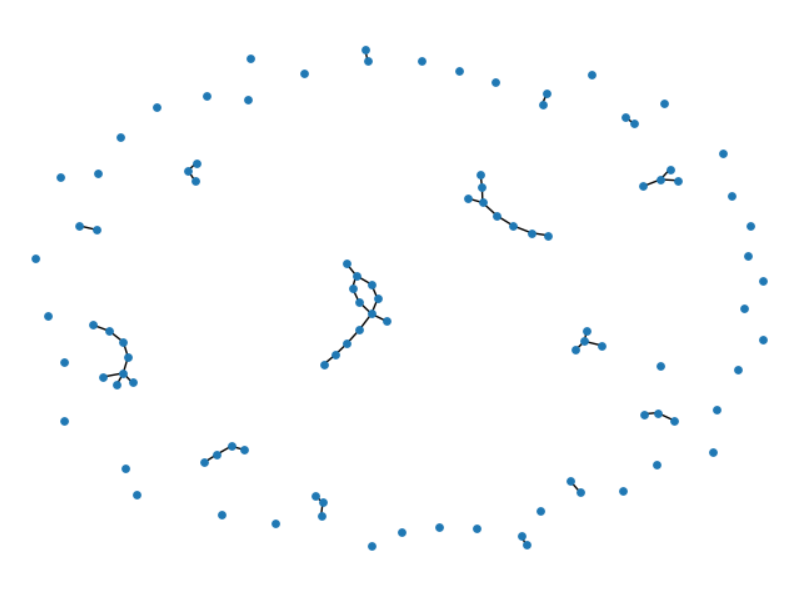
\includegraphics[width=\linewidth]{image/E_R_N100_p0,01.png}
    \end{subfigure}
    \hfill
    \begin{subfigure}[t]{0.49\textwidth}
        \centering
        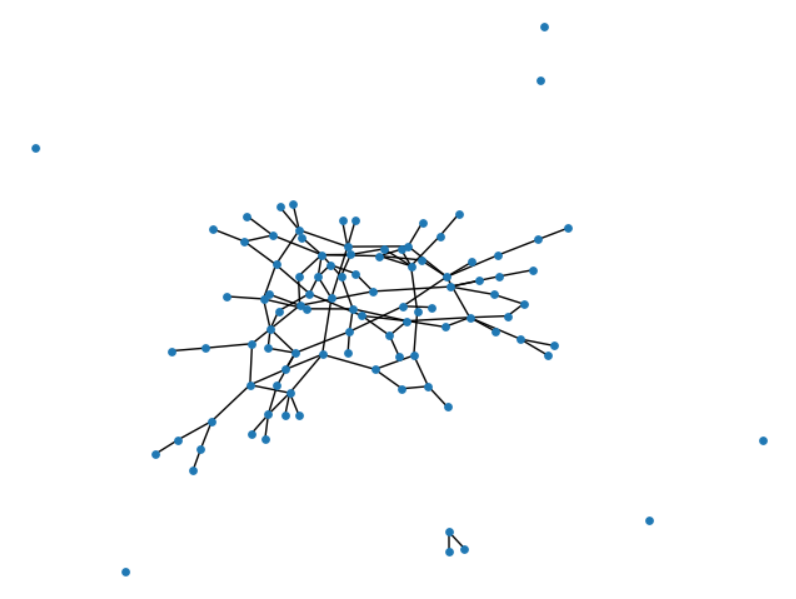
\includegraphics[width=\linewidth]{image/E_R_N100_p0,02.png}
    \end{subfigure}
    \caption{Two examples of Erd\H{o}s-Rényi random graphs: on the left, it has 100 nodes and $p = 0.01$; on the right, it has 100 nodes and $p = 0.02$. Overcoming the threshold $p > 0.01$ can be seen the formation of the giant component.}
    \label{E-R_example}
\end{figure}
%the algorithm is define as below :
%\begin{enumerate}
 %   \item we identify the graph by its adjacency matrix;
 %   \item For each possible link, we generate a random number, if it is less than $p$ the respective entry in the adjacency matrix  is 1 otherwise 0.
%\end{enumerate}

However, the E-R algorithm does not produce networks similar to those found in nature which tend to be more clustered and to have hubs (nodes with very high degree). To simulate these properties, new algorithms have been proposed like the Barab\'abi-Albert scale-free network and the Watts-Strogatz small-world network.

\subsection{Barab\'abi-Albert Scale-Free Network}
Barab\'abi and Albert (B-A) proposed a scale-free network $G(N, m)$, where $N$ is the number of nodes and $m$ is a parameter, that mimics the behavior of real graph like the Internet \cite{Barabasi_Albert_1999}. This type of graph exhibits some preferential nodes which have a degree order of magnitude higher than the average and it presents a power law as degree distribution.
The model works by preferential attachment, where new nodes are more likely to connect to nodes that already have a higher degree. 

The algorithm is defined as follow:
\begin{enumerate}
    \item It is initialized a complete graph of $m_0 > m$ node, usually $m_0 = m+1$;
    \item The other nodes are connected to this graph: for each new node, it is connected to $m$ nodes with probability $p_i = \frac{k_i}{\sum_i k_i}$, where $k_i$ is the degree of the $i$ node.
\end{enumerate}
Figure \ref{B-A_example} shows two examples of B-A networks.

\begin{figure}[ht!]
    \centering
    \begin{subfigure}[t]{0.49\textwidth}
        \centering
        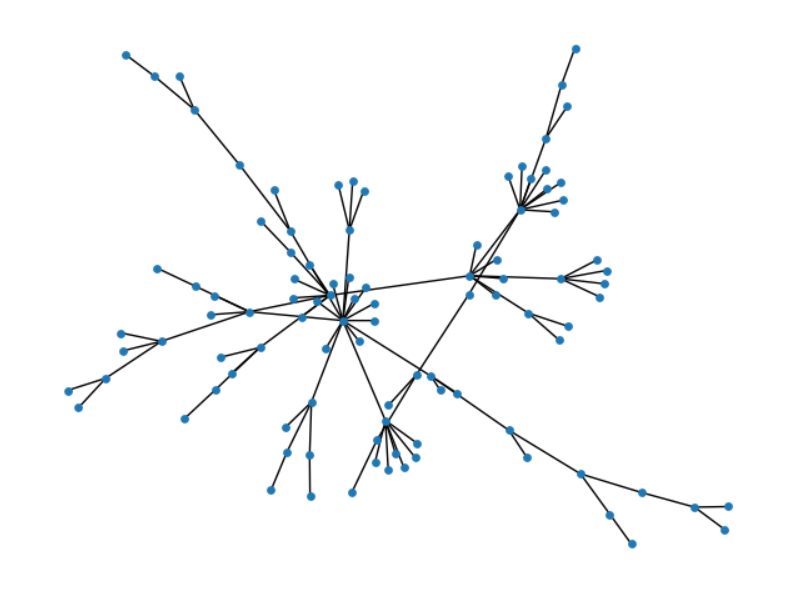
\includegraphics[width=\linewidth]{image/B_A_N100_m1.png}
    \end{subfigure}
    \hfill
    \begin{subfigure}[t]{0.49\textwidth}
        \centering
        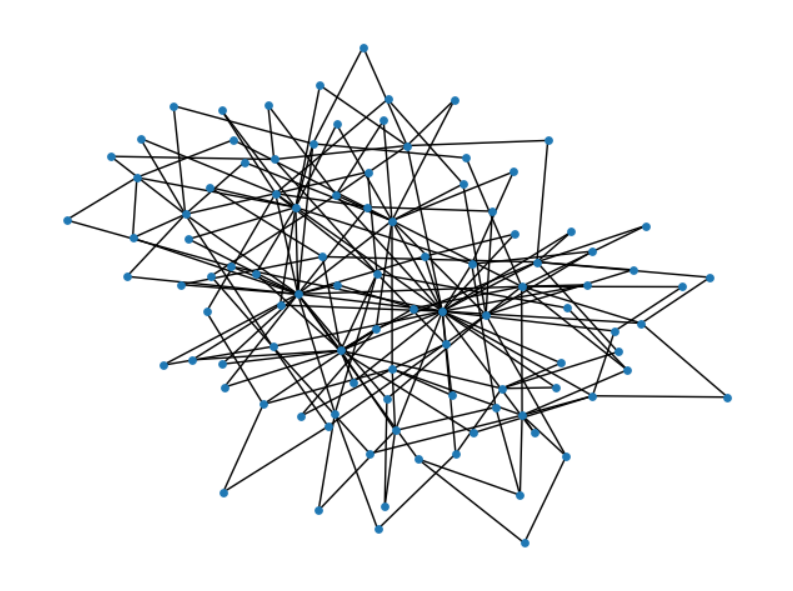
\includegraphics[width=\linewidth]{image/B_A_N100_m2.png}
    \end{subfigure}
    \caption{Two example of Barab\'abi-Albert scale-free networks: on the left, it has 100 nodes and $m=1$; on the right, it has 100 nodes and $m=2$.}
    \label{B-A_example}
\end{figure}

\subsection{Watts-Strogatz Small World Network}

The Watts-Strogatz small-world network $G(N, K, p)$, where $N$ is the number of nodes, $K$ is the average degree (it must be even) and $p$ is the rewiring probability, is a model that exhibits high clustering and short average path lengths \cite{Watts-Strogatz_1998}. The degree distribution follows a power law and the network is homogeneous, meaning that all nodes have similar degree.

The algorithm is defined as follows:
\begin{enumerate}
    \item A ring network with $N$ nodes is created, where each node is connected to the $K/2$ nearest neighbors on each side;
    \item For each edge, with probability $p$ the link is removed and a new one is created to random node. There is no preferential attachments. The new link must be a not existing one.
\end{enumerate}

Figure \ref{W-S_example} it shows two example of W-S networks.

\begin{figure}[ht!]
    \centering
    \begin{subfigure}[t]{0.49\textwidth}
        \centering
        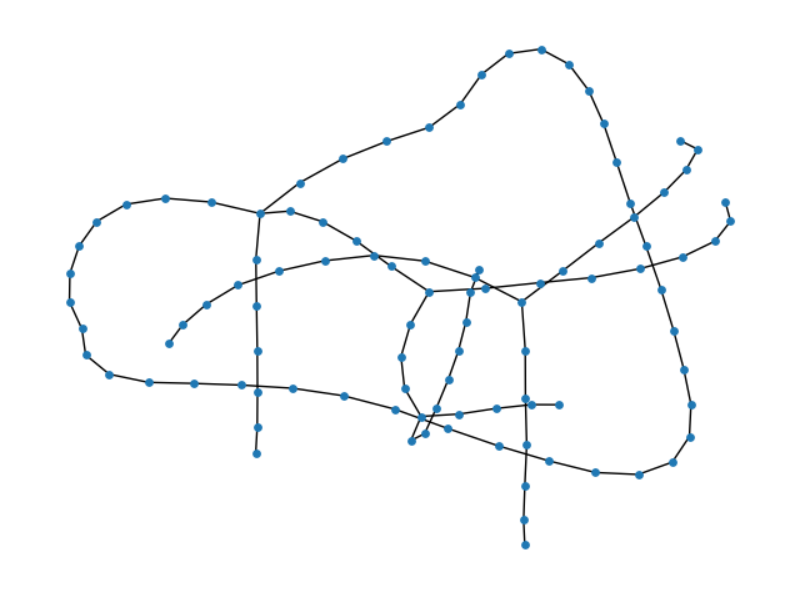
\includegraphics[width=\linewidth]{image/W_S_N100_K2_p0,1.png}
    \end{subfigure}
    \hfill
    \begin{subfigure}[t]{0.49\textwidth}
        \centering
        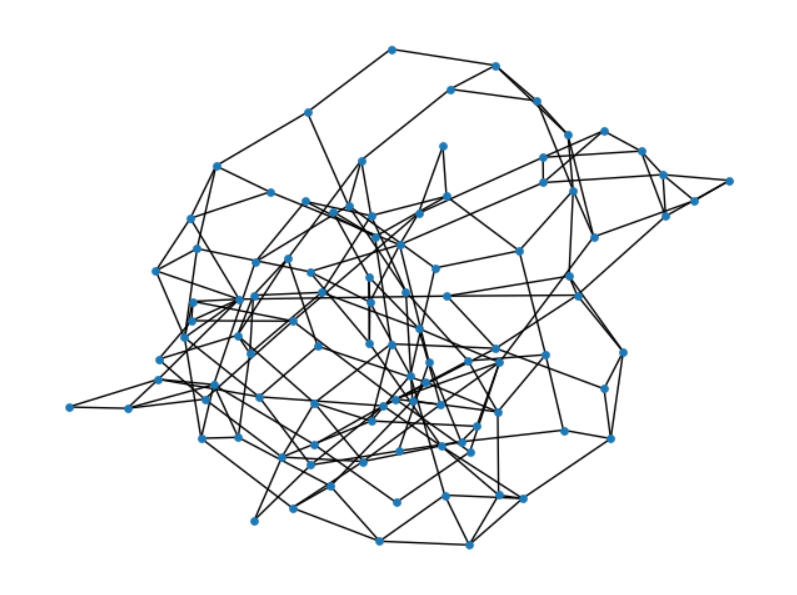
\includegraphics[width=\linewidth]{image/W_S_N100_K4_p0,3.png}
    \end{subfigure}
    \caption{Two example of Watts-Strogatz small world networks: on the left, it has 100 nodes, $K=2$ and $p=0.1$; on the right, it has 100 nodes, $K=4$ and $p=0.3$.}
    \label{W-S_example}
\end{figure}

The B-A and W-S algorithms produce more realistic networks compared to the E-R one, but both focus on their specific feature: the B-A networks fail to reproduce the high clustering of real networks and the W-S ones fail to reproduce the hubs characteristic of networks like Internet.

\section{Random Walk on Networks}

The study of random walks on networks is fundamental in understanding various dynamical processes, such as diffusion, search algorithms, and transport phenomena. In this section, we formalize the mathematical framework of random walks on networks and explore their key properties, including stationary distributions, transition probabilities, and their connection to the Laplacian matrix.

Consider a network $G(N,M)$ where a particle moves randomly between the nodes at each time step, with transition probability $P_{ij}$ to go to the node $j$ starting from the node $i$. If the link between them does not exist then $P_{ij}= 0$. 
The dynamics of this system behaves as a Markov chain: it has no memory of the past states and the future state depends only on the current position.
Let $\rho_i(n)$ be the probability of finding the particle at the node $i$ at time step $n$. The discrete time evolution of the system is given by the law
\begin{equation}
    \rho_i(n+1) = \sum_j P_{ij}\rho_j(n).
\end{equation}

In order to conserve the total probability the transition probability must be a stochastic matrix, namely it must hold 
\begin{equation}
    \sum_i P_{ij}(\Delta t) = 1 .
\end{equation}

The transition probability can be identified with the adjacency matrix of the network
\begin{equation}
    P_{ij} = \frac{A_{ij}}{\sum_j A_{ij}}.
\end{equation}

If the system holds the detailed balance condition
\begin{equation}\label{detail_condition}
    \pi_{ij} \rho_j^* = \pi_{ji} \rho_i^*
\end{equation}
the system admits a unique stationary solution $\rho^*$ such that
\begin{equation}
    \sum_j P_{ij}\rho^*_j =  \rho^*_i .
\end{equation}
This can be written in matrix formalism, where $\Pi$ is the matrix of the transition probability and $\rho^*(t)$ is the stationary probability vector, as
\begin{equation}
    \Pi \rho^* = \rho^*.
\end{equation}
Tus, the stationary distribution is the eigenvector corresponding to the eigenvalue $1$ of the transition matrix.


Taking the continuum limit, we obtain the master equation \cite{Classic_random_walk}
\begin{equation}\label{master_eq}
    \dot \rho_i(t) = \sum_j \pi_{ij}\rho_j(t) - \pi_{ji}\rho_i(t) = - \sum_j L_{ij} \rho_j(t),
\end{equation}
where $\pi_{ij}$ is the transition rate, namely the transition probability per units of time, and $L_{ij} = \sum_k \pi_{kj}\delta_{ij} -\pi_{ij} $ is the Laplacian matrix.
The first term represents incoming transitions to node $i$, while the second term accounts for outgoing transitions.

The Laplacian matrix has the property that $L_{ij} < 0 $ for $i \neq j$ and also it satisfies the relation
\begin{equation}
    \sum_i L_{ij} = 0 .
\end{equation} 

The eigenvalues of the Laplacian matrix have always a not negative real part and its spectrum contains at least one zero eigenvalue, therefore it is not invertible \cite{Boccaletti}. The multiplicity of the zero eigenvalue is equal to the number of connected component of the network: in fact that if the network is not connected the Laplacian should be a block matrix,  block for each connected component, each component can be seen as an independent network with their zero eigenvalue.

The solution of master equation \eqref{master_eq} is
\begin{equation}\label{random_walk_solution}
    \rho(t) = e^{-tL}\rho(0).
\end{equation}

The master equation, in the matrix formalism, for the stationary distribution reduces to 
\begin{equation}\label{stationary_distribution}
    \dot \rho^*(t) = -L \rho^*(t) = 0 . 
\end{equation}
Thus, the stationary distribution is the eigenvector with eigenvalue $0$ of the Laplacian matrix. 
%The other eigenvalues are connected to the Ljapunov exponent and to the time that the occurs to converge to $\rho^*$.

We can prove that
\begin{equation}
    \sum_i \dot\rho_i(t) = - \sum_i \sum_j L_{ij} \rho_j(t) = - \sum_j \left(\sum_i L_{ij}\right) \rho_j(t) = 0 .
\end{equation}
This implies a first integral of motion 
\begin{equation}
    \sum_i \rho_i(t) = \sum_i \rho_i(0) .
\end{equation}

%%add the part with the measure of the eigenvalue, i.e. sum_{\lamda \neq 0} v_\lambda(t) = 0

Let us now assume the network satisfies the detailed balance condition \eqref{detail_condition}, then there exists a hyperplane $\Sigma_0$ that is orthogonal to the stationary distribution and this subspace is invariant under the dynamics. Let be $w \in \Sigma_0$, this subspace is identify by the relation
\begin{equation}
    \sum_i w_i = 0 
\end{equation}
As a matter of fact, let $w(t) \in \Sigma_0$ then 
\begin{equation}
    \sum_i w_i(t+1) = \sum_{ij} \pi_{ij} w_j(t) = \sum_j \underbrace{\left(\sum_i \pi_{ij}\right)}_{1} w_j = \sum_j w_j(t) = 0.
\end{equation}

Therefore, any probability vector can be decomposed as a direct sum of the stationary state and a vector $w(t) \in \Sigma_0$ 
\begin{equation}
    \rho(t) = \rho^* + w(t).
\end{equation}

Furthermore, if the detailed balance condition holds \eqref{detail_condition}, the stationary distribution  is \cite{Classic_random_walk}
\begin{equation}
    \rho^* = \frac{1}{N} \left(1,1,\cdots,1,1\right).
\end{equation} 

The uncertainty in the particle's location can be captured by the Shannon entropy
\begin{equation}
    S = -\sum_i p_i\ln p_i.
\end{equation}
It is a bounded function $0\geq S \geq \ln N$.
It can been shown that the stationary distribution maximizes the Shannon entropy $S = \ln N$.
    
\begin{comment}
    In figure \ref{fig:node_0} is shown only the probability to be in the initial node as a function of time starting  from a Dirac delta distribution for different types of networks\footnote{The python scripts can be found in the GitHub page of the author at the link: \url{https://github.com/ShqemzaMatteo/Master_thesis}}: a ring graph, an Erd\H{o}s-Rényi (E-R) random graph\cite{erdos-renyi1960}, a Barab\'asi-Albert (B-A) scale-free graph\cite{Barabasi_Albert_1999}, and a Watts-Strogatz (W-S) small-sworld graph\cite{Watts-Strogatz_1998}. All the algorithm are explained in the Appendix \Ref{Appendix_A}. 

    \begin{figure}[ht!]
        \centering
        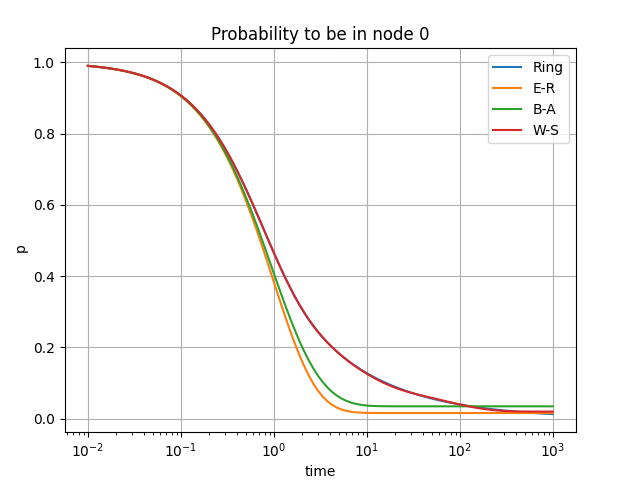
\includegraphics[width=0.65\linewidth]{image/random_graph_node_0.png}
        \caption{Plot of the probability $p$ to be in the node 0 starting from a Dirac delta distribution or the same node as a function of time for different network types of $50$ nodes: a ring graph (blue), a Erd\H{o}s-Rényi (E-R) random graph with connectivity probability $0.7$ (orange), a Barab\'asi-Albert (B-A) scale-free graph with parameter $m=3$ (green), and a Watts-Strogatz (W-S) small world graph with parameter $K=3$ and rewire probability 0.2 (red).}
        \label{fig:node_0}
    \end{figure}
\end{comment}

\section{Quantum Walk}
We can extend the random walk model to quantum particles. 
They must follow the Schrödinger equation with the Laplacian as Hamiltonian. However, the Schrödinger equation requires that the Laplacian is hermitian; therefore, the network must hold the detailed balance condition \eqref{detail_condition}.
This model is known as “continuos time quantum walk" \cite{Farhi_98, quantum_walk}. This model is used to build quantum algorithms \cite{Quantum_walk_Google, classic_to_quantum_networks}.

Let us define an orthonormal basis $\{\ket{i}\}$, where each element $\ket{i}$ indicates their corresponding node $i$, satisfying $\braket{i}{j}=\delta_{ij}$. 
A general general state of the network can be encoded in the ket state $\ket{\psi}$ is define as
\begin{equation}\label{ket_state_quantum}
    \ket{\psi} = \sum_i \sqrt{\rho_i(t)} \ket{i},
\end{equation}
in this way $\rho_i = |\braket{i}{\psi}|^2$ is the projection of the state in the node $i$, in other words the probability that the system can be measured in the node $i$. The norm of $\ket{\psi}$ is normalize to $1$, therefore, the projections $\rho_i$ satisfy the condition $\sum_i \rho_i = 1$.
The Schrödinger equation can be written as
\begin{equation}\label{Schrödinger_quantum_walk}
    \frac{d}{dt}\ket{\psi} = -i\frac{1}{2}\hat L\ket{\psi}.
\end{equation}
where $\hat L = \sum_{ij} L_{ij}\ket{i}\bra{j}$ is the Laplacian operator.
If we apply a Wick rotation into the equation \eqref{Schrödinger_quantum_walk} we recover the master equation of the classic random walk \eqref{master_eq}.

The solution of the equation \eqref{Schrödinger_quantum_walk} takes the form
\begin{equation}
    \ket{\psi(t)} = \hat U(t,0) \ket{\psi(0)} = e^{-\frac{i}{2}\hat L t} \ket{\psi(0)},
\end{equation}
where $\hat U(t,t') =e^{-\frac{i}{2}\hat L (t-t')}$ is the evolution operator and now it is unitary. It holds the following property: $\hat U(t,t')\hat U(t',t'') = U(t,t'')$.

It is possible to define a limiting transition probability for a quantum walk as follow: suppose the system starts at node $\ket{a}$, we measure it after a time $t$, random variable uniformly distributed over the interval $t \in [0,T]$ \cite{quantum_walk}. The transition probability from node $a$ to $b$ is given by
\begin{equation}
    \begin{split}
        \rho_{a\rightarrow b}(T) &= \frac{1}{T}\int_0^T |\bra{a}e^{-i\frac{t}{2}\hat L} \ket{b}|^2 dt\\
        &=\frac{1}{T}\int_0^T \sum_{\lambda,\lambda'}\bra{a}e^{i\frac{t}{2}\hat L}\ket{\lambda}\braket{\lambda}{b} \bra{b}e^{-i\frac{t}{2}\hat L} \ket{\lambda'}\braket{\lambda'}{a} dt\\
        &= \sum_{\lambda,\lambda'}\braket{a}{\lambda}\braket{\lambda}{b}\braket{b}{\lambda'}\braket{\lambda'}{a}\frac{1}{T}\int_0^T e^{-i(\lambda-\lambda')\frac{t}{2}}dt\\
        &= \sum_\lambda|\braket{a}{\lambda}\braket{\lambda}{b}|^2+2\sum_{\lambda\neq\lambda'}\braket{a}{\lambda}\braket{\lambda}{b}\braket{b}{\lambda'}\braket{\lambda'}{a}\frac{1-e^{-i(\lambda-\lambda')\frac{T}{2}}}{i(\lambda-\lambda')T},\\
    \end{split}
\end{equation}
where $\ket{\lambda}$ are the eigenstates of $\hat L$ with eigenvalues $\lambda$. In the limit $T\rightarrow \infty$ it tend to 
\begin{equation}
    \rho_{a\rightarrow b}(T) \xrightarrow[T \rightarrow \infty]{} \sum_\lambda|\braket{a}{\lambda}\braket{\lambda}{b}|^2.
\end{equation}

Let the system be in the state $\ket{\psi}$, also called pure state, we can define the density matrix as
\begin{equation}
    \hat\rho =\ket{\psi}\bra{\psi} = \sum_{ij} \sqrt{\rho_i} \sqrt{\rho_j}\ket{i}\bra{j},
\end{equation}
It is a self-adjoint operator and $\Tr[\hat\rho] = 1$ \cite{Nielsen_Chuang_2010}.

For a generic operator $\hat O(t) = O_{ij}\ket{i}\bra{j}$, the expectation value of the respective observable can be found as
\begin{equation}
        \left< \hat O\right> = \Tr\left[\hat O\hat\rho\right].
\end{equation}
The probability $\rho_k$ to be in the node $k$ can be express using the operator $\hat P_k = \ket{k}\bra{k}$ such that
\begin{equation} \label{state_projection_quantum}
    \begin{split}
        \Tr\left[\hat P_k\hat\rho(t)\right] 
        %= \sum_i \braket{i}{a}\braket{a}{\psi}\braket{\psi}{i}
        %& = \sum_{ijk} \braket{i}{a}\bra{a}\sqrt{\rho_j}\ket{j}\bra{k}\sqrt{\rho_k}\ket{i}\\
        %&= \sum_{ijk} \delta_{i,a}\delta_{a,j}\delta_{k,i}\sqrt{\rho_j}\sqrt{\rho_k}\\
        %= \sqrt{\rho_a}\sqrt{\rho_a} 
        = \rho_k.
    \end{split}
\end{equation}

In the Heisenberg picture, the density operator evolution can be found solving the different equation called Von Neumann equation
\begin{equation}\label{Von Neumann equation}
    \begin{split}
        \frac{d}{dt}\hat\rho(t) 
        %&= \frac{d}{dt}\left(\ket{\psi(t)}\bra{\psi(t)}\right) = \\
        %&= -\frac{i}{2}\hat L\ket{\psi(t)}\bra{\psi(t)} + \ket{\psi(t)}\bra{\psi(t)}\frac{i}{2}\hat L\\
        &= -\frac{i}{2}\left[\hat L,\rho\right]
    \end{split}
\end{equation}
where $[\cdot,\cdot]$ is the commutator.
The solution of the differential equation is
\begin{equation}
    \hat\rho(t) = \hat U(t,0)\hat\rho(0)\hat U^\dagger(t,0) = e^{-\frac{i}{2}t\hat L}\hat\rho\, e^{\frac{i}{2}t\hat L}.
\end{equation}

Using the cyclic property of the trace and the unity of the evolution operator, it can be proved that the $\Tr[\hat\rho]$ is time invariant.

If the initial distribution over the network is uncertain, we can introduce the density matrix for mixed state. Let be $\{\ket{\psi_k}\}_{k<K\in\mathbb{R}}$ a set of different probability state that can describe the system with probability $p_k$, such that $\sum_k^K p_k = 1$, then the mixed density matrix is define as
\begin{equation}
    \hat \rho = \sum_{k=1}^K p_k \hat \rho_k \qquad \hat\rho_k = \ket{\psi_k}\bra{\psi_k}.
\end{equation}

The temporal evolution of the operator is defined as in eq. \eqref{Von Neumann equation}; the probability to be at node a at time t is the same as in eq. \eqref{state_projection_quantum}. All the property for the pure state still holds; this can be easily proven using the linearity of the trace.

Using the mixed density matrix we can consider a system that does not start from a defined distribution, but from an ensemble of possible distribution with their probability. 

To study the mixed state we introduce the Von Neumann entropy
\begin{equation}\label{Von_Neumann_entropy}
    S[\hat\rho]=-\Tr[\hat\rho\ln\hat\rho].
\end{equation}
It is the quantum counterpart of the Shannon entropy for classical information theory.
The Von Neumann entropy \eqref{Von_Neumann_entropy} is bounded $0\geq S[\hat\rho] \geq \ln N$. It vanishes for pure states.
The Von Neumann entropy is a time invariance, thus, the evolution operator takes pure state into pure state \cite{Nielsen_Chuang_2010}.
\begin{comment}
    \begin{equation}
        \begin{split}
            S[\hat\rho(t)] &=\Tr[\hat\rho(t)\ln\hat\rho(t)]= \Tr[U(t,0)\hat\rho(t)U^\dagger(t,0)\ln\left(U(t,0)\hat\rho(t)U^\dagger(t,0)\right)]\\
            &=\Tr[U(t,0)\hat\rho(0)U^\dagger(t,0)U(t,0)\ln\left(\hat\rho(0)\right)U^\dagger(t,0)]\\
            &= S[\hat\rho(0)].
        \end{split}
    \end{equation}
    We can move out the evolution operator because they are unitary, since if we consider the taylor expansion
    \begin{equation}
        \begin{split}
            \ln\left(U(t,0)\hat\rho(t)U^\dagger(t,0)\right) &= c_0U(t,0)U^\dagger(t,0) + c_1 U(t,0)\hat\rho(t)U^\dagger(t,0)\\
            & \quad + c_2 U(t,0)\hat\rho(t)U^\dagger(t,0)U(t,0)\hat\rho(t)U^\dagger(t,0) + ... \\
            &=  U(t,0)\ln\left(\hat\rho(t)\right) U^\dagger(t,0).
        \end{split}
    \end{equation}
\end{comment}

\begin{comment}
If we consider the system in contact with a thermal bath with which exchange only energy but conserving it in average, namely the canonical condition hold, there is a stationary state $\hat\rho = e^{-\beta \hat L}$ that maximize the entropy. The parameter $\beta$ is just the inverse of a pseudo-temperature that stands for the interaction with the thermal bath. 
Since the thermal bath actively changes the entries of $\hat L$, it is changing the weight of the network and the probability to move from node $i$ to $j$. Thus, we are considering a network that is changing randomly by time. 
The reader can recognize that this density matrix is the same the De Domenico has introduced \eqref{density_matrix}.
\end{comment}

\subsection{1-D Quantum Random Walk}
Consider a toy model: the quantum random walk over a discrete line \cite{Farhi_98}. The probability of moving left or right is $\frac{1}{2}$.
To analyze this model, it is useful to introduce the momentum state $\ket{p}$ such that $\braket{j}{p} = e^{ijp}$, where $-\pi < p< \pi$.

In line the Laplacian is defined as
\begin{equation}
    \hat L \ket{j} = 2\ket{j} -\ket{j-1} -\ket{j+1} . 
\end{equation}
Therefore, applying this to the momentum state
\begin{equation}
    \begin{split}
        \bra{j}\hat L \ket{p} &= \braket{j}{p} -\frac{1}{2}\braket{j-1}{p} -\frac{1}2{}\braket{j+1}{p}\\
        &= e^{ijp} -\frac{1}{2}e^{i(j-1)p} - \frac{1}{2}e^{i(j+1)p}\\
        &= e^{ijp}(\cos(p) - 1) = (\cos(p) - 1)\braket{j}{p}
    \end{split}
\end{equation}

Thus, the amplitude of the walk can be computed as the integral over all the momenta, leading to
\begin{equation}
    \begin{split}
        \bra{j}e^{-i\frac{t}{2}\hat L} \ket{k}&= \frac{1}{2\pi}\int_{-\pi}^{\pi} e^{-i\frac{t}{2}(\cos(p) - 1)} \braket{j}{p} \braket{p}{k} dp\\
        &= \frac{1}{2\pi}\int_{-\pi}^{\pi} e^{-ip(j-k)-i\frac{t}{2}(\cos(p) - 1)}\\
        & = e^{i\frac{t}{2}}(-i)^{k-j}J_{k-j}\left(\frac{t}{2}\right),
   \end{split}
\end{equation}
where $J_{n}(x)$ is the Bessel function of the first kind of order $n$.

Applying the Wick rotation we obtain 
\begin{equation}\label{Bessel_function}
    \left|\bra{j}e^{-i\frac{t}{2}\hat L} \ket{k}\right|^2 = e^{-t} \left(I_{k-j}\left(\frac{t}{2}\right)\right)^2,
\end{equation}
where $I_{n}(x) = i^{n}J_{n}(ix)$ is the modified Bessel function of the first kind.
In the limit $t\gg 1$ it tends to a gaussian centered in the origin and variance $\sqrt{t}$, in accordance with the classical model \cite{mabramowitz64:handbook}.

\subsection{Double tree network}
Another important toy model is the quantum walk on a network consisting of two binary trees of depth $n$ with the ending connected as shown in figure \ref{fig:Double_Tree}.
We start from one root and analyze the probability to reach the other one \cite{quantum_walk}.
Classically, the probability of crossing the network scales exponentially as $2^{-n}$, and it is not computable for big $n$.
However, using the quantum version it remains computable.
\begin{figure}[ht!]
    \centering
    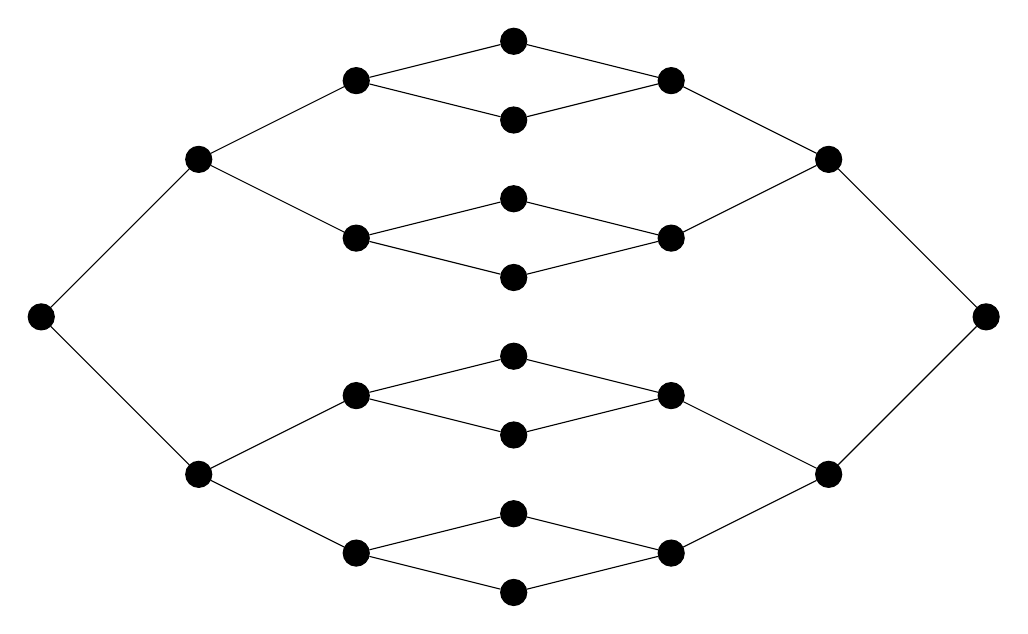
\begin{tikzpicture}[>=stealth, node distance=2cm, every node/.style={circle, draw, fill=black}]
        %draw nodes by coordinates
        \node (n00) at (-6,0) {};
        \node (n11) at (-4,2) {};
        \node (n12) at (-4,-2) {};
        \node (n21) at (-2,3) {};
        \node (n22) at (-2,1) {};
        \node (n23) at (-2,-1) {};
        \node (n24) at (-2,-3) {};
        \node (n31) at (0,3.5) {};
        \node (n32) at (0,2.5) {};
        \node (n33) at (0,1.5) {};
        \node (n34) at (0,0.5) {};
        \node (n35) at (0,-0.5) {};
        \node (n36) at (0,-1.5) {};
        \node (n37) at (0,-2.5) {};
        \node (n38) at (0,-3.5) {};
        \node (n41) at (2,3) {};
        \node (n42) at (2,1) {};
        \node (n43) at (2,-1) {};
        \node (n44) at (2,-3) {};
        \node (n51) at (4,2) {};
        \node (n52) at (4,-2) {};
        \node (n60) at (6,0) {};
        
        % Draw edges (links)
        \draw (n00) -- (n11);
        \draw (n00) -- (n12);
        \draw (n11) -- (n21);
        \draw (n11) -- (n22);
        \draw (n12) -- (n23);
        \draw (n12) -- (n24);
        \draw (n21) -- (n31);
        \draw (n21) -- (n32);
        \draw (n22) -- (n33);
        \draw (n22) -- (n34);
        \draw (n23) -- (n35);
        \draw (n23) -- (n36);
        \draw (n24) -- (n37);
        \draw (n24) -- (n38);
        \draw (n31) -- (n41);
        \draw (n32) -- (n41);
        \draw (n33) -- (n42);
        \draw (n34) -- (n42);
        \draw (n35) -- (n43);
        \draw (n36) -- (n43);
        \draw (n37) -- (n44);
        \draw (n38) -- (n44);
        \draw (n41) -- (n51);
        \draw (n42) -- (n51);
        \draw (n43) -- (n52);
        \draw (n44) -- (n52);
        \draw (n51) -- (n60);
        \draw (n52) -- (n60);
    \end{tikzpicture}
    \caption{The picture of a glued double tree network.}
    \label{fig:Double_Tree}
\end{figure}

To simplify the analysis, we can introduce a new basis $\ket{\mathrm{col}\; j}_{j<2n}$ that indicates a column and not the single node, except at the two root nodes where they coincide. This basis is defined as
\begin{equation}
    \ket{\mathrm{col}\; j} = \frac{1}{\sqrt{N_j}}\sum_{a\in \mathrm{column}} \ket{a}, 
\end{equation}
where the renormalization factor $N_j$ is 
\begin{equation}
    N_j = \left\{\begin{aligned}
        &2^j \qquad &0\leq j\leq n\\
        &2^{2n-j} \qquad &n \leq j \leq 2n
    \end{aligned}\right. .
\end{equation}

In this basis, the Laplacian act as
\begin{equation}
    \begin{aligned}
        \bra{\mathrm{col}\; j}\hat L \ket{\mathrm{col}\; j} &= 1\\
        \bra{\mathrm{col}\; j \pm 1}\hat L \ket{\mathrm{col}\; j} &=\left\{\begin{aligned}
            \frac{\sqrt{2}}{2} \qquad j=0,n,2,\\
            \frac{\sqrt{2}}{3} \qquad \mathrm{otherwise}\\
        \end{aligned}\right.
    \end{aligned}
\end{equation}

Thus, the dynamics along the network reduces to a 1-D quantum walk which has a known computable solution \eqref{Bessel_function} %\cite{quantum_walk}
\begin{equation}
    \bra{0}e^{i\frac{t}{2}\hat L}\ket{2n} = e^{-t} I_{2n}\left(\frac{t}{2}\right),
\end{equation}
where $I_{n}(x) = i^{n}J_{n}(ix)$ is the modified Bessel function of the first kind. 
